\documentclass[UTF8]{ctexart}
\usepackage{algpseudocode}
\usepackage{algorithm}
\usepackage{amsmath}
\usepackage{diagbox}
\usepackage{float}
\usepackage{hyperref}
\usepackage{multirow}
\usepackage{subcaption}
\usepackage{graphicx}
\usepackage[bottom=6em, top=6em]{geometry}
\usepackage{lmodern}
\usepackage{listings}
\usepackage[table]{xcolor}

\ctexset{ section = { format={\Large \bfseries } } }

\definecolor{color1}{rgb}{0.85, 1, 0.85}
\definecolor{color2}{rgb}{1, 0.85, 0.85}
\newcolumntype{g}{>{\columncolor{color1}}p{4.2em}<{\centering}}
\newcolumntype{a}{>{\columncolor{color2}}p{4.2em}<{\centering}}


\title{《可视计算与交互概论》课程大作业报告}
\author{屠学畅}
\date{}

\pagestyle{empty}

\begin{document}

\maketitle

\thispagestyle{empty}

\section{选题}

我选择的题目是 SVG 渲染器。SVG 是一种用于描述二维矢量图形的图形格式,矢量图相比位图拥有许多优点,在特定场景中有着广泛的应用。由于我对 Web 相关技术比较感兴趣,而 SVG 与 Web 结合紧密,我选择了 CPU 上的 SVG 渲染器作为大作业的题目。也正是因为 SVG 可以结合 CSS 等标准,完整的渲染器实现难度较大,我选择了一部分功能实现,最终可以在一些简单的 SVG 文件上得到令人满意的结果。

\section{实现思路}

\subsection{总体过程}

首先,SVG 是基于 XML 的标记语言,因此需要解析 XML 文本。由于解析 XML 并非该题目的核心内容,我调用了第三方库 \href{https://github.com/leethomason/tinyxml2}{TinyXML2}。

得到 SVG 文件的结构后,我从 \texttt{width}、\texttt{height} 和 \texttt{viewBox} 三个参数,结合窗口大小计算得到画布的尺寸和偏移量,使得画布在不超出窗口的前提下尽量大。随后,解析出 \texttt{line}、\texttt{rect}、\texttt{polyline}、\texttt{polygon}、\texttt{circle}、\texttt{ellipse}、\texttt{path} 这几类元素分别进行内部和轮廓的渲染。渲染时即按照 XML 文本的先后顺序依次渲染、覆盖,这也是 SVG 标准规定的元素覆盖关系。

对于除 \texttt{circle} 以外的其它元素,我都使用了与 \texttt{polygon} 类似的原理进行绘制。其中比较复杂的是 \texttt{path} 元素,因为它包含了多种直线和曲线的组合。直线的处理是容易的,对于二阶和三阶的 Bézier 曲线以及椭圆的圆弧,我使用了自适应的细分方法得到折线对于曲线的近似,最终将 \texttt{path} 元素转化为多条折线进行绘制。具体实现方法会在下面介绍。

对于 \texttt{circle} 元素(虽然也可以转化为 \texttt{path}),需要绘制的区域总是形如一个圆环(可能退化为圆),我采用的方法是对于画布中每一列计算与圆的交点,并对有效区域进行绘制。

\subsection{核心方法:闭合折线的填充}

我使用的方法是,枚举画布的每一列,计算该列与折线中的每条线段是否有交,如果有交则记录交点位置,将所有交点位置排序后就容易得到哪些区间是需要填充的了。这里根据 \texttt{fill-rule} 选项有两种不同的规则 \texttt{evenodd} 和 \texttt{nonzero},但在实现上不存在本质区别。

为了优化运行效率,应当避免无效的枚举,因此我使用了扫描线的方法,使用 \texttt{std::set} 动态地维护与当前枚举的列相交的线段集合,极大提升了速度。

\subsection{折线的轮廓}

由于 SVG 中的轮廓有指定的宽度,在宽度较大时本质也是填充的过程,因此将每条线段向着法线方向扩展一个宽度的距离得到的新线段连接起来就是要填充的闭合折线。对于连接处的处理,我实现了 \texttt{stroke-linejoin} 选项中的默认值 \texttt{miter}。

\subsection{其他细节}

\begin{itemize}
    \item 项目在课程 Lab 框架的基础上实现。
    \item 以上的绘制过程中只考虑了像素在或不在区域内两种情况,会出现锯齿,我实现了超采样的方法,可以选择以两倍或三倍尺寸渲染,再将若干像素平均,可以较好地避免锯齿的出现。但是这样会大大增加运行时间。
    \item 在 UI 中显示了分辨率和渲染用时。
    \item 实现了带 $\alpha$ 通道的颜色叠加。
    \item 列优先的渲染顺序缓存不友好,因此我翻转了渲染时的画布,在降采样阶段再翻转回来。
    \item 在曲线的绘制中,求出参数方程的形式后,取出中点对于两段曲线递归细分,直到端点距离近到无法在当前渲染的精度下分辨为止。
    \item 实现了矩形 \texttt{rect} 的圆角效果。
    \item 更多细节可以参考 \texttt{src/VCX/Lab/Project} 目录下的代码,有较为完整的注释。
\end{itemize}

\section{算法亮点}

算法实现了基础的 SVG 元素的渲染、超采样、半透明颜色叠加等功能,在测试样例中可以以较好的运行效率达到接近完美的结果。算法没有参考其它成熟或实验性的渲染器实现。

\section{编译环境}

与 Lab 框架一致,增加了 TinyXML2 库(Xmake 有收录)。可以使用 \texttt{xmake} 进行编译,使用 \texttt{xmake run project} 运行。

\section{测试样例展示}

测试平台:Windows 11,Intel Core i7-12700H。

图片标题中,\underline{$561 \times 1079$ $(\times 2)$, 13ms} 表示显示尺寸为 $561 \times 1079$,实际渲染尺寸为 $1122 \times 2158$,用时 13ms。

\begin{figure}[H]
    \centering
    \begin{subfigure}[b]{0.9\textwidth}
        \centering
        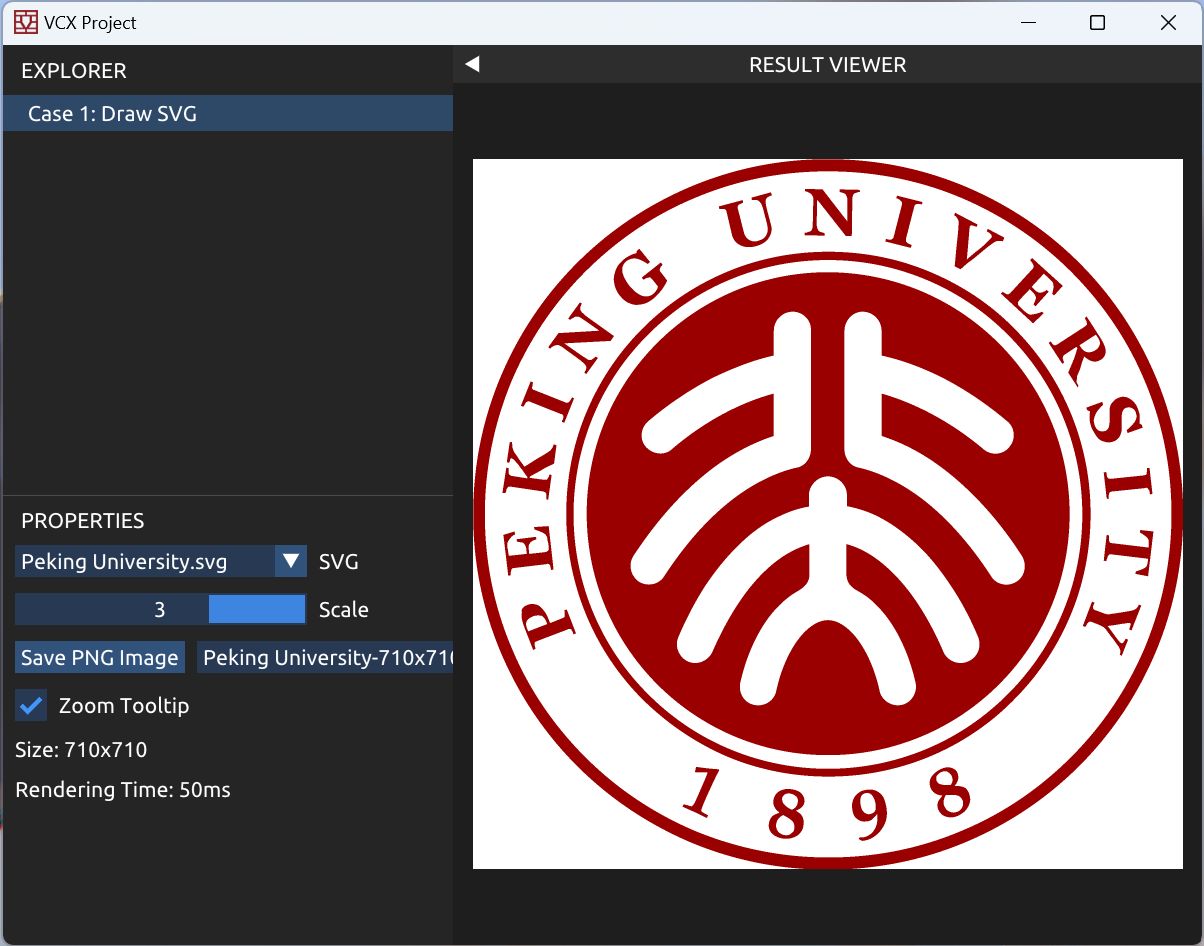
\includegraphics[width=\textwidth]{images/Screenshot.png}
        \caption{UI}
    \end{subfigure}
    \par\bigskip
    \begin{subfigure}[b]{0.3\textwidth}
        \centering
        
\includegraphics[width=\textwidth]{images/Basic Shapes-532x1024-x2-13ms.png}
        \caption{Basic Shapes: \\$532 \times 1024$ $(\times 2)$, 13ms}
    \end{subfigure}
    \hfill
    \begin{subfigure}[b]{0.6\textwidth}
        \centering
        
\includegraphics[width=\textwidth]{images/Peking University-1024x1024-x2-44ms.png}
        \caption{Peking University: \\$1024 \times 1024$ $(\times 2)$, 44ms}
    \end{subfigure}
\end{figure}

\begin{figure}[H]
    \ContinuedFloat
    \centering
    \begin{subfigure}[b]{\textwidth}
        \centering
        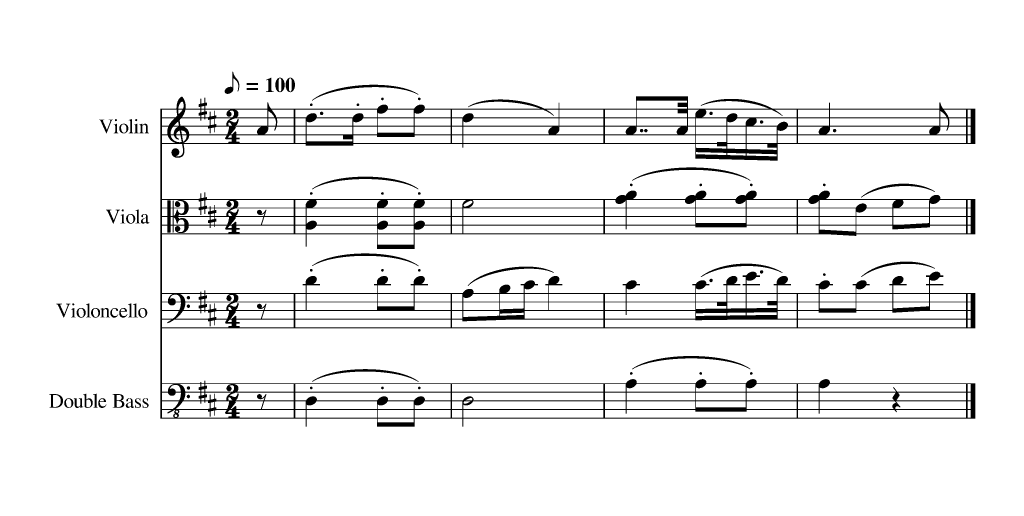
\includegraphics[width=\textwidth]{images/Score-1024x516-x3-150ms.png}
        \caption{Score: \\$1024 \times 516$ $(\times 3)$, 150ms}
    \end{subfigure}
    \par\bigskip
    \begin{subfigure}[b]{0.45\textwidth}
        \centering
        
\includegraphics[width=\textwidth]{images/TikTok-1024x298-x2-14ms.png}
        \caption{TikTok: \\$1024 \times 298$ $(\times 2)$, 14ms}
    \end{subfigure}
    \hfill
    \begin{subfigure}[b]{0.45\textwidth}
        \centering
        
\includegraphics[width=\textwidth]{images/Google-1024x346-x2-21ms.png}
        \caption{Google: \\$1024 \times 346$ $(\times 2)$, 21ms}
    \end{subfigure}
    \par\bigskip
    \begin{subfigure}[b]{0.45\textwidth}
        \centering
        
\includegraphics[width=\textwidth]{images/Microsoft-1024x218-x2-15ms.png}
        \caption{Microsoft: \\$1024 \times 218$ $(\times 2)$, 15ms}
    \end{subfigure}
    \hfill
    \begin{subfigure}[b]{0.45\textwidth}
        \centering
        
\includegraphics[width=\textwidth]{images/Handwritten Text-1024x398-x2-15ms.png}
        \caption{Handwritten Text: \\$1024 \times 398$ $(\times 2)$, 15ms}
    \end{subfigure}
    \par\bigskip
    \begin{subfigure}[b]{0.45\textwidth}
        \centering
        
\includegraphics[width=\textwidth]{images/Evenodd-1024x384-x2-17ms.png}
        \caption{Evenodd: \\$1024 \times 384$ $(\times 2)$, 17ms}
    \end{subfigure}
    \hfill
    \begin{subfigure}[b]{0.45\textwidth}
        \centering
        
\includegraphics[width=\textwidth]{images/Nonzero-1024x384-x2-17ms.png}
        \caption{Nonzero: \\$1024 \times 384$ $(\times 2)$, 17ms}
    \end{subfigure}
\end{figure}

\begin{figure}[H]
    \ContinuedFloat
    \centering
    \begin{subfigure}[b]{0.6\textwidth}
        \centering
        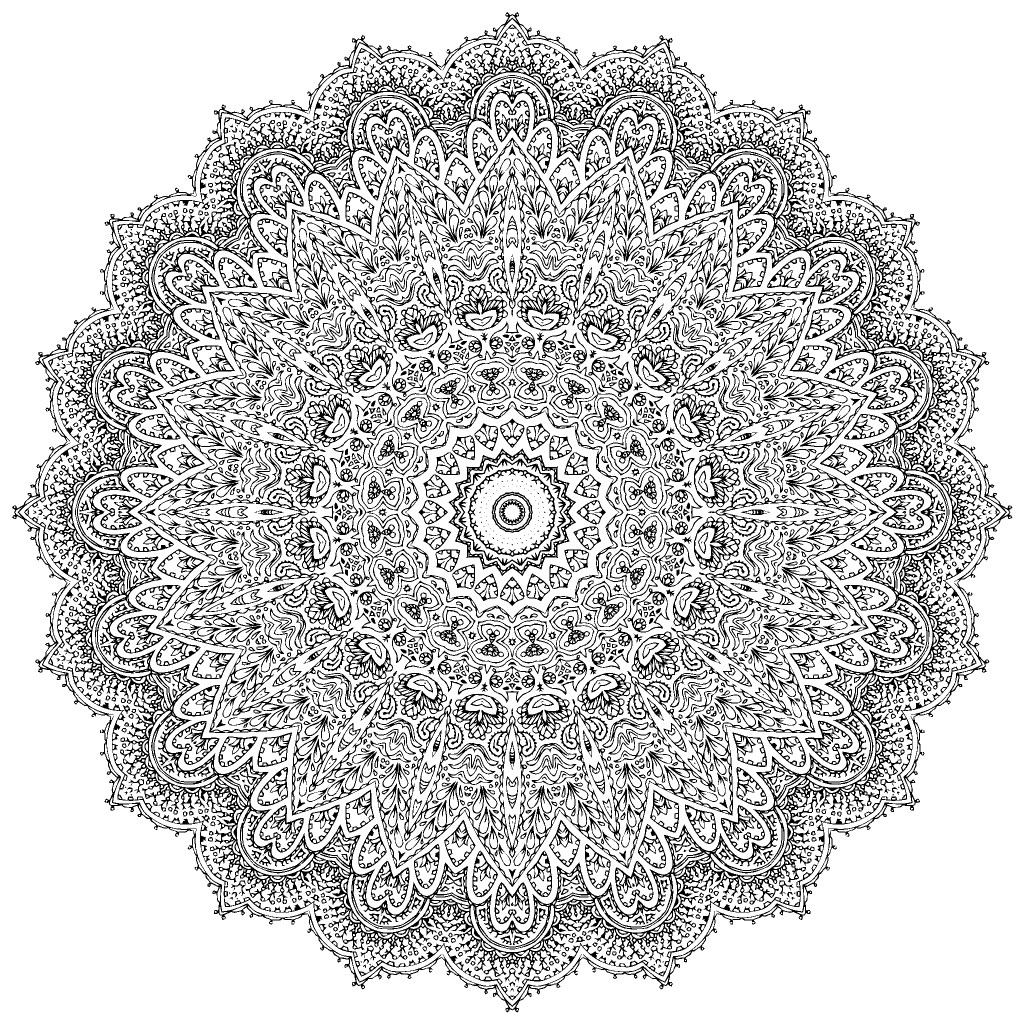
\includegraphics[width=\textwidth]{images/Mandala-1024x1024-x2-496ms.png}
        \caption{Mandala: \\$1024 \times 1024$ $(\times 2)$, 496ms}
    \end{subfigure}
    \hfill
    \begin{subfigure}[b]{0.3\textwidth}
        \centering
        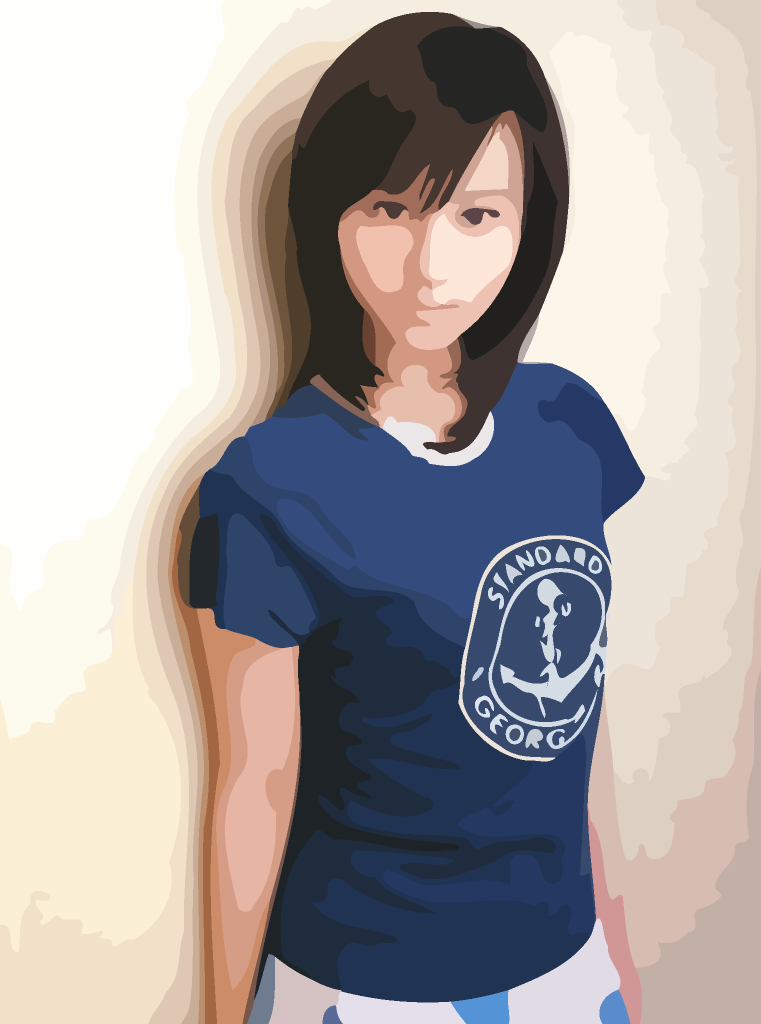
\includegraphics[width=\textwidth]{images/Girl-761x1024-x2-111ms.png}
        \caption{Girl: \\$761 \times 1024$ $(\times 2)$, 111ms}
    \end{subfigure}
    \par\bigskip
    \begin{subfigure}[b]{0.4\textwidth}
        \centering
        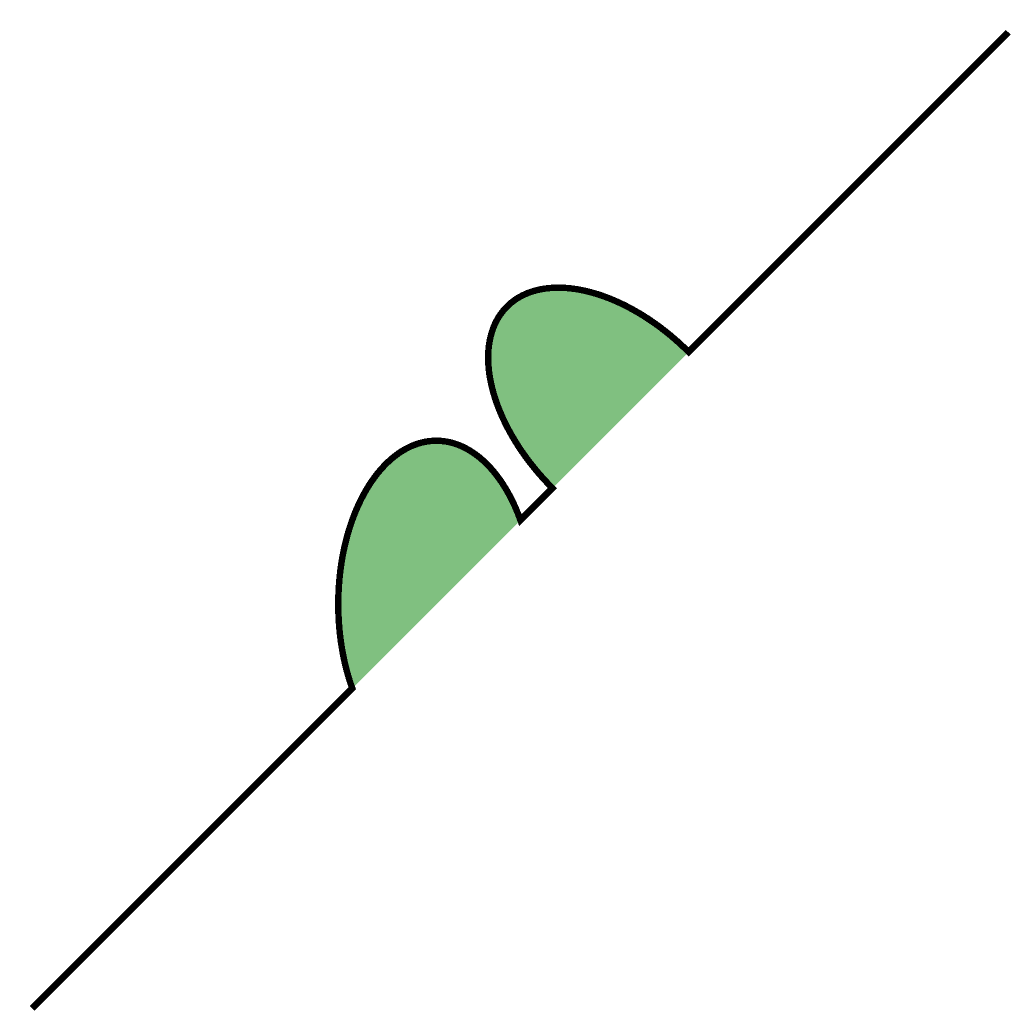
\includegraphics[width=\textwidth]{images/Arcs-1024x1024-x2-19ms.png}
        \caption{Arcs: \\$1024 \times 1024$ $(\times 2)$, 19ms}
    \end{subfigure}
    \hfill
    \begin{subfigure}[b]{0.4\textwidth}
        \centering
        
\includegraphics[width=\textwidth]{images/Twitter-1024x842-x2-55ms.png}
        \caption{Twitter: \\$1024 \times 842$ $(\times 2)$, 55ms}
    \end{subfigure}
    \par\bigskip
    \begin{subfigure}[b]{0.6\textwidth}
        \centering
        
\includegraphics[width=\textwidth]{images/Opacity-1024x256-x2-19ms.png}
        \caption{Opacity: \\$1024 \times 256$ $(\times 2)$, 19ms}
    \end{subfigure}
    \caption{测试样例}
\end{figure}

以上测试达到了与浏览器渲染 SVG 相同的效果,速度也比较理想。

下表统计了三张图片在不同分辨率下的渲染用时,单位为毫秒。其中\colorbox{color1}{绿色列}表示总用时,\colorbox{color2}{红色列}表示删去与 \texttt{Common::ImageRGB} 交互的部分后的用时,如果这个值相比前者小很多,则表明大量的时间花费在逐个像素的赋值上。每个值均是五次测试的平均值。由于 Twitter.svg 不是正方形,实际高度约为 82\%。

\vspace{2em}
\bgroup
\def\arraystretch{1.3}
\begin{center}
\begin{tabular}{|c|g|a|g|a|g|a|}
    \hline
     & \multicolumn{2}{c|}{Twitter.svg} & \multicolumn{2}{c|}{Peking University.svg} & \multicolumn{2}{c|}{Mandala.svg} \\
    \cline{2-7}
    \hline
    $256 \times 256$ & 1 & 0 & 3 & 2 & 302 & 276 \\
    \hline
    $512 \times 512$ & 3 & 0 & 5 & 3 & 292 & 289 \\
    \hline
    $768 \times 768$ & 8 & 1 & 8 & 4 & 311 & 306 \\
    \hline
    $1024 \times 1024$ & 14 & 2 & 12 & 5 & 331 & 325 \\
    \hline
    $2048 \times 2048$ & 56 & 7 & 44 & 14 & 431 & 416 \\
    \hline
    $4096 \times 4096$ & 223 & 27 & 162 & 38 & 654 & 591 \\
    \hline
\end{tabular}
\end{center}
\egroup
\vspace{2em}

这三张图片依次可以代表简单、普通和复杂的情形。可以看到,在前两种情况下,性能的瓶颈在于逐像素的赋值,如果需要继续改进,应当首先考虑更改与引擎交互的方式。对于第三张图片,的确是渲染器的算法导致了性能瓶颈。

以下是文件的来源。
\begin{itemize}
    \item Basic Shapes: \href{https://developer.mozilla.org/en-US/docs/Web/SVG/Tutorial/Basic\_Shapes}{\texttt{https://developer.mozilla.org/en-US/docs/Web/SVG/Tutorial/\\Basic\_Shapes}}。
    \item Peking University: \href{https://commons.wikimedia.org/wiki/File:Peking_University_seal.svg}{\texttt{https://commons.wikimedia.org/wiki/File:Peking\_Univers\\ity\_seal.svg}},因为没有实现 CSS 的解析,使用了 Adobe Illustrator 将颜色信息嵌入元素。
    \item Score: 使用 MuseScore 4 导出,片段为 Piano Quintet in A major, D.667 第四乐章的开头(这里确实没钢琴)。
    \item TikTok: \href{https://en.wikipedia.org/wiki/File:TikTok_logo.svg}{\texttt{https://en.wikipedia.org/wiki/File:TikTok\_logo.svg}}。
    \item Google: \href{https://commons.wikimedia.org/wiki/File:Google_2015_logo.svg}{\texttt{https://commons.wikimedia.org/wiki/File:Google\_2015\_logo.svg}}。
    \item Microsoft: \href{https://commons.wikimedia.org/wiki/File:Microsoft_logo_(2012).svg}{\texttt{https://commons.wikimedia.org/wiki/File:Microsoft\_logo\_(2012).\\svg}}。
    \item Handwritten Text: 在 iPad 上使用 GoodNotes 自己写的。
    \item Evenodd、Nonzero: \href{https://developer.mozilla.org/en-US/docs/Web/SVG/Attribute/fill-rule}{\texttt{https://developer.mozilla.org/en-US/docs/Web/SVG/Attri\\bute/fill-rule}}。
    \item Mandala: \href{https://pixabay.com/zh/vectors/mandala-vintage-classic-retro-2031287/}{\texttt{https://pixabay.com/zh/vectors/mandala-vintage-classic-retro-2\\031287/}}。
    \item Girl: \href{https://commons.wikimedia.org/wiki/File:HM_04_lowdetail.svg}{\texttt{https://commons.wikimedia.org/wiki/File:HM\_04\_lowdetail.svg}}。
    \item Arcs: \href{https://developer.mozilla.org/en-US/docs/Web/SVG/Tutorial/Paths}{\texttt{https://developer.mozilla.org/en-US/docs/Web/SVG/Tutorial/Paths}}。
    \item Twitter: \href{https://commons.wikimedia.org/wiki/File:Twitter-logo.svg}{\texttt{https://commons.wikimedia.org/wiki/File:Twitter-logo.svg}}。
    \item Opacity: \href{https://developer.mozilla.org/en-US/docs/Web/SVG/Attribute/stroke-opacity}{https://developer.mozilla.org/en-US/docs/Web/SVG/Attribute/stroke-opa\\city}
\end{itemize}


\section{对实验结果的思考}

SVG 标准的内容非常多,本次实验只尝试实现了其中很小的一部分,但许多细节已经非常复杂。各种元素格式的解析,虽然难度不高,但却是比较繁琐的。实际上找一张新的图片来测试,它很有可能无法显示正确的结果。

我先后尝试了多种画线的算法,但由于有宽度参数,我最终选择统一转化为多边形的填充。作为核心的多边形填充除了使用扫描线优化(较大尺寸时大约提升了 3 到 5 倍的速度,不严谨)并没有做本质上的更改,因为效果以及非极端情况下的效率已经令人满意了。

另一个关键的问题是 anti-aliasing,我只实现了超采样的方法。但是对于一般的 SVG 图片,绝大部分区域是纯色色块(除非使用了 \texttt{<linearGradient>} 等元素),一个显然的改进是针对边缘区域进行超采样,对纯色区域则不做改变,甚至可以降低分辨率。其它抗锯齿方法也有进一步探索的价值。



\end{document}